% ======================================================================
% ICAIIC 2027 submission (English). IEEE conference format, max 6 pages.
%
% EVERY measured number in this file is a macro from numbers.tex, which is
% generated (together with checks of every qualitative claim) by
%       sh tools/build_paper.sh      (or: python -m tools.paper_numbers)
% Never type a measured number here by hand. Literal figures are limited to
% configuration constants (10 s window, 5 s hop, 500 ms tick, tau = 0.80,
% sample counts of the explainers) and to numbers quoted from other papers
% or from our offline study (marked OFFLINE below).
% ======================================================================
\documentclass[conference]{IEEEtran}
\IEEEoverridecommandlockouts

\usepackage[T1]{fontenc}
\usepackage[utf8]{inputenc}
\usepackage{amsmath,amssymb}
\usepackage{booktabs}
\usepackage{array}
\usepackage{xspace}
\usepackage{url}
\usepackage{tikz}
\usetikzlibrary{arrows.meta,positioning,fit}
\usepackage[hidelinks]{hyperref}

% AUTO-GENERATED by tools/paper_numbers.py -- do not edit by hand.
% data version: v1
\newcommand{\DataVersion}{v1\xspace}
\newif\ifvone \vonetrue
\newcommand{\LoopClosedLagPNF}{661\xspace}  % 15_v2/loop_check/fog_t_closed_shap.json
\newcommand{\LoopClosedLagMax}{730\xspace}
\newcommand{\LoopClosedN}{11\xspace}
\newcommand{\LoopOpenLagPNF}{20\xspace}  % 15_v2/loop_check/fog_t_open_shap.json
\newcommand{\LoopOpenLagMax}{270\xspace}
\newcommand{\LoopOpenN}{11\xspace}
\newcommand{\ColocNoneRespMed}{7.3\xspace}  % 07_edge_xai/edge_xai_none.json
\newcommand{\ColocNoneRespPNF}{9.7\xspace}
\newcommand{\ColocNoneExecMed}{5.8\xspace}
\newcommand{\ColocNoneXaiMed}{\textbf{??}\xspace}
\newcommand{\ColocNoneNet}{0.7\xspace}
\newcommand{\ColocNoneRSS}{187\xspace}
\newcommand{\ColocNoneCPU}{0.6\xspace}
\newcommand{\ColocNoneN}{44\xspace}
\newcommand{\ColocShapCRespMed}{462.0\xspace}  % 07_edge_xai/edge_xai_shapucuz.json
\newcommand{\ColocShapCRespPNF}{511.1\xspace}
\newcommand{\ColocShapCExecMed}{460.4\xspace}
\newcommand{\ColocShapCXaiMed}{445\xspace}
\newcommand{\ColocShapCNet}{0.8\xspace}
\newcommand{\ColocShapCRSS}{493\xspace}
\newcommand{\ColocShapCCPU}{8.2\xspace}
\newcommand{\ColocShapCN}{44\xspace}
\newcommand{\ColocLimeCRespMed}{352.8\xspace}  % 07_edge_xai/edge_xai_limeucuz.json
\newcommand{\ColocLimeCRespPNF}{585.0\xspace}
\newcommand{\ColocLimeCExecMed}{351.5\xspace}
\newcommand{\ColocLimeCXaiMed}{346\xspace}
\newcommand{\ColocLimeCNet}{0.6\xspace}
\newcommand{\ColocLimeCRSS}{431\xspace}
\newcommand{\ColocLimeCCPU}{7.7\xspace}
\newcommand{\ColocLimeCN}{44\xspace}
\newcommand{\ColocLimeRespMed}{690.0\xspace}  % 07_edge_xai/edge_xai_lime.json
\newcommand{\ColocLimeRespPNF}{1{,}177.0\xspace}
\newcommand{\ColocLimeExecMed}{688.5\xspace}
\newcommand{\ColocLimeXaiMed}{682\xspace}
\newcommand{\ColocLimeNet}{0.7\xspace}
\newcommand{\ColocLimeRSS}{448\xspace}
\newcommand{\ColocLimeCPU}{15.2\xspace}
\newcommand{\ColocLimeN}{44\xspace}
\newcommand{\ColocShapRespMed}{1{,}154.5\xspace}  % 07_edge_xai/edge_xai_shap.json
\newcommand{\ColocShapRespPNF}{1{,}833.3\xspace}
\newcommand{\ColocShapExecMed}{1{,}152.4\xspace}
\newcommand{\ColocShapXaiMed}{1{,}143\xspace}
\newcommand{\ColocShapNet}{1.0\xspace}
\newcommand{\ColocShapRSS}{523\xspace}
\newcommand{\ColocShapCPU}{23.7\xspace}
\newcommand{\ColocShapN}{44\xspace}
\newcommand{\ColocHW}{Intel x86-64, 20 cores\xspace}
\newcommand{\ColocStack}{Py 3.11.9, torch 2.8.0+cpu\xspace}
\newcommand{\ColocRAM}{16\xspace}
\newcommand{\ColocKbps}{187\xspace}
\newcommand{\FogNoneRespMed}{10.6\xspace}  % 04_fog/fog_xai_none.json
\newcommand{\FogNoneRespPNF}{42.2\xspace}
\newcommand{\FogNoneExecMed}{3.5\xspace}
\newcommand{\FogNoneXaiMed}{\textbf{??}\xspace}
\newcommand{\FogNoneNet}{3.5\xspace}
\newcommand{\FogNoneRSS}{210\xspace}
\newcommand{\FogNoneCPU}{0.0\xspace}
\newcommand{\FogNoneN}{44\xspace}
\newcommand{\FogShapCRespMed}{442.6\xspace}  % 04_fog/fog_xai_shapucuz.json
\newcommand{\FogShapCRespPNF}{574.0\xspace}
\newcommand{\FogShapCExecMed}{394.1\xspace}
\newcommand{\FogShapCXaiMed}{390\xspace}
\newcommand{\FogShapCNet}{24.2\xspace}
\newcommand{\FogShapCRSS}{422\xspace}
\newcommand{\FogShapCCPU}{5.0\xspace}
\newcommand{\FogShapCN}{44\xspace}
\newcommand{\FogLimeCRespMed}{645.2\xspace}  % 04_fog/fog_xai_limeucuz.json
\newcommand{\FogLimeCRespPNF}{802.5\xspace}
\newcommand{\FogLimeCExecMed}{588.1\xspace}
\newcommand{\FogLimeCXaiMed}{584\xspace}
\newcommand{\FogLimeCNet}{28.5\xspace}
\newcommand{\FogLimeCRSS}{442\xspace}
\newcommand{\FogLimeCCPU}{10.8\xspace}
\newcommand{\FogLimeCN}{44\xspace}
\newcommand{\FogLimeRespMed}{1{,}227.5\xspace}  % 04_fog/fog_xai_lime.json
\newcommand{\FogLimeRespPNF}{1{,}407.1\xspace}
\newcommand{\FogLimeExecMed}{1{,}158.1\xspace}
\newcommand{\FogLimeXaiMed}{1{,}154\xspace}
\newcommand{\FogLimeNet}{34.7\xspace}
\newcommand{\FogLimeRSS}{449\xspace}
\newcommand{\FogLimeCPU}{22.8\xspace}
\newcommand{\FogLimeN}{44\xspace}
\newcommand{\FogShapRespMed}{1{,}456.2\xspace}  % 04_fog/fog_xai_shap.json
\newcommand{\FogShapRespPNF}{1{,}548.5\xspace}
\newcommand{\FogShapExecMed}{1{,}431.1\xspace}
\newcommand{\FogShapXaiMed}{1{,}426\xspace}
\newcommand{\FogShapNet}{12.5\xspace}
\newcommand{\FogShapRSS}{464\xspace}
\newcommand{\FogShapCPU}{25.9\xspace}
\newcommand{\FogShapN}{44\xspace}
\newcommand{\FogHW}{Intel x86-64, 12 cores\xspace}
\newcommand{\FogStack}{Py 3.14.7, torch 2.14.0+cpu\xspace}
\newcommand{\FogRAM}{16\xspace}
\newcommand{\FogKbps}{187\xspace}
\newcommand{\CloudNoneRespMed}{63.5\xspace}  % 13_bulut/cloud_taban_3tur.json
\newcommand{\CloudNoneRespPNF}{154.5\xspace}
\newcommand{\CloudNoneExecMed}{4.1\xspace}
\newcommand{\CloudNoneXaiMed}{\textbf{??}\xspace}
\newcommand{\CloudNoneNet}{29.7\xspace}
\newcommand{\CloudNoneRSS}{518\xspace}
\newcommand{\CloudNoneCPU}{0.4\xspace}
\newcommand{\CloudNoneN}{\textbf{??}\xspace}
\newcommand{\CloudShapCRespMed}{429.8\xspace}  % 13_bulut/cloud_xai_shapucuz.json
\newcommand{\CloudShapCRespPNF}{509.0\xspace}
\newcommand{\CloudShapCExecMed}{343.6\xspace}
\newcommand{\CloudShapCXaiMed}{340\xspace}
\newcommand{\CloudShapCNet}{43.1\xspace}
\newcommand{\CloudShapCRSS}{797\xspace}
\newcommand{\CloudShapCCPU}{7.2\xspace}
\newcommand{\CloudShapCN}{44\xspace}
\newcommand{\CloudLimeCRespMed}{463.3\xspace}  % 13_bulut/cloud_xai_limeucuz.json
\newcommand{\CloudLimeCRespPNF}{608.3\xspace}
\newcommand{\CloudLimeCExecMed}{344.3\xspace}
\newcommand{\CloudLimeCXaiMed}{340\xspace}
\newcommand{\CloudLimeCNet}{59.4\xspace}
\newcommand{\CloudLimeCRSS}{751\xspace}
\newcommand{\CloudLimeCCPU}{3.5\xspace}
\newcommand{\CloudLimeCN}{44\xspace}
\newcommand{\CloudLimeRespMed}{870.1\xspace}  % 13_bulut/cloud_xai_lime.json
\newcommand{\CloudLimeRespPNF}{1{,}091.8\xspace}
\newcommand{\CloudLimeExecMed}{747.6\xspace}
\newcommand{\CloudLimeXaiMed}{744\xspace}
\newcommand{\CloudLimeNet}{61.2\xspace}
\newcommand{\CloudLimeRSS}{764\xspace}
\newcommand{\CloudLimeCPU}{14.7\xspace}
\newcommand{\CloudLimeN}{44\xspace}
\newcommand{\CloudShapRespMed}{1{,}300.5\xspace}  % 13_bulut/cloud_xai_shap.json
\newcommand{\CloudShapRespPNF}{1{,}715.8\xspace}
\newcommand{\CloudShapExecMed}{1{,}173.3\xspace}
\newcommand{\CloudShapXaiMed}{1{,}169\xspace}
\newcommand{\CloudShapNet}{63.6\xspace}
\newcommand{\CloudShapRSS}{838\xspace}
\newcommand{\CloudShapCPU}{15.2\xspace}
\newcommand{\CloudShapN}{44\xspace}
\newcommand{\CloudHW}{DO-Regular, 1 core\xspace}
\newcommand{\CloudStack}{Py 3.11.16, torch 2.14.0+cu130\xspace}
\newcommand{\CloudRAM}{2\xspace}
\newcommand{\CloudKbps}{187\xspace}
\newcommand{\FogXaiOverExecLow}{111\xspace}  % min xai / none exec
\newcommand{\FogXaiOverExecHigh}{404\xspace}
\newcommand{\FogXaiMinMs}{390\xspace}
\newcommand{\FogXaiMaxMs}{1{,}426\xspace}
\newcommand{\FogRespGrowth}{137\xspace}
\newcommand{\FogNoneHopPct}{0.07\xspace}  % none exec / 5 s hop
\newcommand{\CloudOverColocNone}{8.69\xspace}
\newcommand{\FogOverColocNone}{1.45\xspace}
\newcommand{\CloudOverColocShapC}{0.93\xspace}
\newcommand{\FogOverColocShapC}{0.96\xspace}
\newcommand{\FogOverColocXaiShapC}{0.88\xspace}
\newcommand{\CloudOverColocLimeC}{1.31\xspace}
\newcommand{\FogOverColocLimeC}{1.83\xspace}
\newcommand{\FogOverColocXaiLimeC}{1.69\xspace}
\newcommand{\CloudOverColocLime}{1.26\xspace}
\newcommand{\FogOverColocLime}{1.78\xspace}
\newcommand{\FogOverColocXaiLime}{1.69\xspace}
\newcommand{\CloudOverColocShap}{1.13\xspace}
\newcommand{\FogOverColocShap}{1.26\xspace}
\newcommand{\FogOverColocXaiShap}{1.25\xspace}
\newcommand{\SelThr}{0.80\xspace}  % 09_secici_xai/fog_sel80_tam.json
\newcommand{\SelN}{1{,}030\xspace}
\newcommand{\SelMinutes}{87\xspace}
\newcommand{\SelNExpl}{145\xspace}
\newcommand{\SelRate}{14.1\xspace}
\newcommand{\SelPerExpl}{365\xspace}
\newcommand{\SelRespMean}{80.1\xspace}
\newcommand{\SelRespMedian}{11.0\xspace}
\newcommand{\SelRespPNF}{446\xspace}
\newcommand{\SelExecMean}{55.3\xspace}
\newcommand{\SelQueueMax}{0.06\xspace}
\newcommand{\AlwRespMean}{450.5\xspace}
\newcommand{\AlwExecMean}{400.2\xspace}
\newcommand{\NonRespMean}{15.9\xspace}
\newcommand{\NonExecMean}{3.59\xspace}
\newcommand{\AlwN}{44\xspace}
\newcommand{\SelSpeedup}{5.6\xspace}
\newcommand{\CapNon}{1{,}394\xspace}  % hop / mean execution
\newcommand{\CapSel}{90\xspace}  % hop / mean execution
\newcommand{\CapAlw}{12\xspace}  % hop / mean execution
\newcommand{\CapGain}{7.5\xspace}
\newcommand{\ProjRespMean}{78.5\xspace}  % selective_xai_sweep_d2
\newcommand{\ProjErr}{2.0\xspace}
\newcommand{\ProjRateErr}{2.3\xspace}
\newcommand{\AccEleven}{0.952\xspace}  % 08_kalibrasyon/calibration_d1.json
\newcommand{\ConfEleven}{0.909\xspace}
\newcommand{\ECEEleven}{0.047\xspace}
\newcommand{\CalNEleven}{604\xspace}
\newcommand{\RateElevenSixty}{6.3\xspace}
\newcommand{\CatchElevenSixty}{37.9\xspace}
\newcommand{\RateElevenSeventy}{10.4\xspace}
\newcommand{\CatchElevenSeventy}{62.1\xspace}
\newcommand{\RateElevenEighty}{14.4\xspace}
\newcommand{\CatchElevenEighty}{89.7\xspace}
\newcommand{\RateElevenNinety}{21.4\xspace}
\newcommand{\CatchElevenNinety}{100.0\xspace}
\newcommand{\ECEtsEleven}{0.256\xspace}
\newcommand{\AccFourteen}{0.690\xspace}  % 08_kalibrasyon/calibration_d1.json
\newcommand{\ConfFourteen}{0.908\xspace}
\newcommand{\ECEFourteen}{0.227\xspace}
\newcommand{\CalNFourteen}{594\xspace}
\newcommand{\RateFourteenSixty}{1.7\xspace}
\newcommand{\CatchFourteenSixty}{2.7\xspace}
\newcommand{\RateFourteenSeventy}{4.4\xspace}
\newcommand{\CatchFourteenSeventy}{6.0\xspace}
\newcommand{\RateFourteenEighty}{11.8\xspace}
\newcommand{\CatchFourteenEighty}{12.0\xspace}
\newcommand{\RateFourteenNinety}{29.3\xspace}
\newcommand{\CatchFourteenNinety}{28.8\xspace}
\newcommand{\ECEtsFourteen}{0.276\xspace}
\newcommand{\FaithShapC}{0.250\xspace}  % 11_pareto/pareto_c5.json
\newcommand{\FaithSemShapC}{0.043\xspace}
\newcommand{\MonoShapC}{0.565\xspace}
\newcommand{\SensShapC}{0.123\xspace}
\newcommand{\FaithLimeC}{0.209\xspace}  % 11_pareto/pareto_c5.json
\newcommand{\FaithSemLimeC}{0.035\xspace}
\newcommand{\MonoLimeC}{0.604\xspace}
\newcommand{\SensLimeC}{0.049\xspace}
\newcommand{\FaithLime}{0.232\xspace}  % 11_pareto/pareto_c5.json
\newcommand{\FaithSemLime}{0.037\xspace}
\newcommand{\MonoLime}{0.579\xspace}
\newcommand{\SensLime}{0.045\xspace}
\newcommand{\FaithShap}{0.263\xspace}  % 11_pareto/pareto_c5.json
\newcommand{\FaithSemShap}{0.044\xspace}
\newcommand{\MonoShap}{0.549\xspace}
\newcommand{\SensShap}{0.128\xspace}
\newcommand{\QualN}{40\xspace}
\newcommand{\SensRatio}{2.7\xspace}
\newcommand{\RtAcc}{0.822\xspace}  % 01_streaming (S11+S14, causal norm)
\newcommand{\RtFOne}{0.694\xspace}
\newcommand{\RtN}{1{,}198\xspace}
\newcommand{\ValFOne}{0.939\xspace}
\newcommand{\NParams}{49{,}890\xspace}
\newcommand{\PayloadBytes}{11{,}553\xspace}  % one 500 ms data frame


\newcommand{\ms}{\,ms\xspace}
\protected\def\x{\ensuremath{\times}\xspace}
\xspaceaddexceptions{\% \x \ms}

\begin{document}

\title{Explanation Is the Bottleneck: Measuring and Gating XAI Cost in
Real-Time Stress Detection on a Raspberry Pi Fog Node}

% AUTHOR BLOCK: add the advisor (name, affiliation, e-mail) before submission.
\author{\IEEEauthorblockN{Sena Cindio\u{g}lu}
\IEEEauthorblockA{Dept.\ of Computer Engineering\\
Y\i ld\i z Technical University, Istanbul, T\"urkiye}}

\maketitle

\begin{abstract}
Post-hoc explanations are routinely attached to wearable stress
classifiers, but the time needed to produce them is rarely measured and, to
our knowledge, has not been measured inside a real-time physiological
monitoring pipeline. We deploy a frozen \NParams-parameter 1D-CNN trained
on WESAD as a TCP client--server system, run its server either co-located
with the client on a laptop or on a Raspberry~Pi~4 fog node, and measure
the seven metrics used in fog-computing studies with an open-loop sensor
client and drift-corrected clock synchronisation. Without explanation, the
server pipeline takes a median of \ColocNoneExecMed\ms per 10\,s window on
the laptop and \FogNoneExecMed\ms on the Pi. A single region-based LIME or
SHAP (GradientExplainer) explanation takes a median of
\ColocXaiMin--\ColocXaiMax\ms on the laptop (four operating points) and
\FogXaiMin--\FogXaiMax\ms on the Pi (two reduced-sample operating points),
i.e.\ \XaiShareMin--\XaiShareMax\% of the execution time. The median one-way
network latency is at most \LatMaxAll\ms, whereas the Pi is
\FogOverColocXaiLimeC\x slower per explanation for LIME with 250 samples
and \FogOverColocXaiShapC\x slower for SHAP with 50 samples, and every
response of the latter exceeds the 1\,s real-time bound. On a
\SelMinutes-minute segment in which \SelShapCRate\% of windows had
confidence below 0.80, explaining only those windows reduced the mean
execution time \SelExecGainMin--\SelExecGainMax\x and raised the throughput
capacity of one worker from \FogShapCCap to \SelShapCCap concurrent users.
Gating directs explanations to errors only where confidence is calibrated:
at the same threshold it explains \CaughtElevenEighty of
\ErrorsElevenEighty misclassified windows of one validation subject but
\CaughtFourteenEighty of \ErrorsFourteenEighty of another.
\end{abstract}

\begin{IEEEkeywords}
explainable AI, fog computing, real-time systems, stress detection, LIME,
SHAP, Raspberry Pi
\end{IEEEkeywords}

% ======================================================================
\section{Introduction}
% ======================================================================

Stress detection from wearable physiological signals is well established
on public datasets such as WESAD~\cite{schmidt2018}, and post-hoc
explanations such as LIME~\cite{ribeiro2016} and SHAP~\cite{lundberg2017}
are now a common companion to the classifier. These explanations are
evaluated almost exclusively for quality. A systematic review of XAI
evaluation explicitly excludes run time from its scope~\cite{nauta2023},
and recent work that explains stress classifiers trained on WESAD reports
neither inference nor explanation time~\cite{almadhor2025}. In a real-time
monitor this omission matters: a new 10\,s window arrives every 5\,s, and
the time spent explaining one window is unavailable to the next window and
to other users of the same server.

Fog-computing studies of physiological monitoring measure precisely such
system-level quantities---latency, queuing delay, execution time, response
time, jitter, bandwidth and resource usage---but without
explanations~\cite{erzurumluoglu2025,tuli2020healthfog}. Conversely, XAI
cost is usually reported without a network or a deployment. This paper
measures both in one budget, on a resource-constrained fog node of the kind
used in those studies. Our contributions are:
\begin{enumerate}
\item An end-to-end measurement of explanation cost inside a TCP
client--server stress detection pipeline at two placements, using the seven
metrics of~\cite{erzurumluoglu2025}, an open-loop load generator and
drift-corrected clock synchronisation (Sec.~\ref{sec:system}).
\item Evidence that explanation accounts for \XaiShareMin--\XaiShareMax\%
of server execution time and that, once it is enabled, placement matters
through compute rather than network (Secs.~\ref{sec:res-cost},
\ref{sec:res-place}).
\item A measured characterisation of confidence-gated explanation on the
fog node---cost, throughput capacity and the queuing of several users---each
matched by a simple analytical model (Secs.~\ref{sec:res-selective},
\ref{sec:res-load}).
\item The calibration condition under which gating directs explanations to
errors, and the cost--stability trade-off between explainer operating
points (Secs.~\ref{sec:res-calib}, \ref{sec:res-quality}).
\end{enumerate}

% ======================================================================
\section{Related Work}
% ======================================================================

\textbf{Fog-based physiological monitoring.} Erzurumluo\u{g}lu et
al.~\cite{erzurumluoglu2025} deploy emotion recognition on DREAMER with a
Raspberry~Pi~4 fog worker and report the seven metrics we adopt.
HealthFog~\cite{tuli2020healthfog} compares placements for cardiac
diagnosis in terms of latency and energy. Neither includes explanations.
El~Rashidy et al.~\cite{elrashidy2025} combine a fog architecture with
LIME and Grad-CAM for emotion recognition but do not report per-window
latency or explanation cost.

\textbf{The cost of explanation.} ShaTS~\cite{shats2025} states an explicit
real-time criterion---an explainer that needs more than 1\,s per window is
unsuitable for real-time use---and shows KernelSHAP violating it. Reported
costs vary by orders of magnitude with hardware, input size and estimator:
KernelSHAP takes seconds to minutes per sample~\cite{warnecke2020,jethani2022},
whereas amortised estimators such as FastSHAP~\cite{jethani2022} trade a
long training phase for millisecond explanations. On a Raspberry~Pi~4,
conditionally triggered SHAP has been reported to add about 195\ms per
prediction in a cold-chain monitoring deployment~\cite{taguta2026}.

\textbf{Selective computation.} Gating computation on softmax confidence is
established for inference through early exits~\cite{teerapittayanon2017}
and confidence cascades~\cite{berestizshevsky2018}, and has been proposed
for explanations as budgeted selective explanation~\cite{paes2024} and as
explanations of rejected samples~\cite{artelt2023}. We do not claim the
mechanism. We characterise it end to end in continuous physiological
monitoring on constrained hardware, where its benefit depends on
calibration~\cite{guo2017}.

% ======================================================================
\section{System and Measurement Method}
\label{sec:system}
% ======================================================================

\begin{figure}[t]
\centering
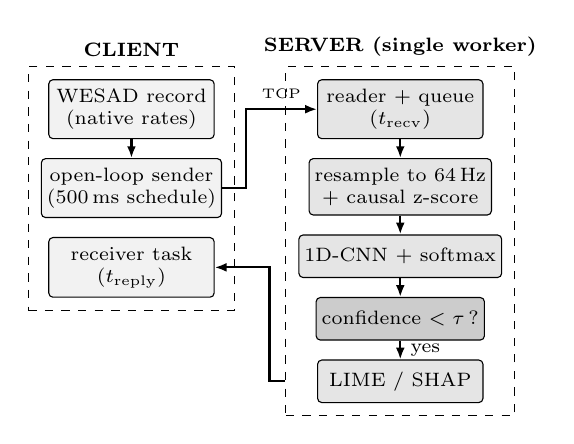
\begin{tikzpicture}[
  node distance=2.4mm,
  blk/.style={draw,rounded corners=1.5pt,align=center,font=\scriptsize,
              minimum height=5.4mm,inner xsep=2pt,minimum width=21mm},
  arr/.style={-{Latex[length=1.5mm]},thick}]
\node[blk,fill=black!5] (rec) {WESAD record\\(native rates)};
\node[blk,fill=black!5,below=of rec] (sch) {open-loop sender\\(500\,ms schedule)};
\node[blk,fill=black!5,below=of sch] (rcv) {receiver task\\($t_\mathrm{reply}$)};
\node[draw,dashed,inner sep=1.6mm,fit=(rec)(sch)(rcv),
      label={[font=\scriptsize\bfseries]above:CLIENT}] (cl) {};
\node[blk,fill=black!10,right=13mm of rec] (q) {reader + queue\\($t_\mathrm{recv}$)};
\node[blk,fill=black!10,below=of q] (pre) {resample to 64\,Hz\\+ causal z-score};
\node[blk,fill=black!10,below=of pre] (cnn) {1D-CNN + softmax};
\node[blk,fill=black!20,below=of cnn] (gate) {confidence $<\tau$\,?};
\node[blk,fill=black!10,below=of gate] (xai) {LIME / SHAP};
\node[draw,dashed,inner sep=1.6mm,fit=(q)(pre)(cnn)(gate)(xai),
      label={[font=\scriptsize\bfseries]above:SERVER (single worker)}] (sv) {};
\draw[arr] (rec) -- (sch);
\draw[arr] (sch.east) -- ++(3mm,0) |- node[pos=0.75,above,font=\tiny]{TCP} (q.west);
\draw[arr] (q) -- (pre);
\draw[arr] (pre) -- (cnn);
\draw[arr] (cnn) -- (gate);
\draw[arr] (gate) -- node[right,font=\scriptsize]{yes} (xai);
\draw[arr] (sv.west |- xai) -- ++(-2mm,0) |- (rcv.east);
\end{tikzpicture}
\caption{Measured pipeline. The explanation is produced by the same worker
as the prediction, so its cost is part of the measured execution and
response times. The server runs either on the client's laptop (co-located)
or on the fog node.}
\label{fig:system}
\end{figure}

\subsection{Model and data}
The classifier is a temporal 1D-CNN with two convolution blocks ([32,\,128]
filters, kernel size 9, BatchNorm--ReLU--MaxPool--Dropout), global average
pooling and two dense layers (\NParams parameters), trained with focal
loss~\cite{lin2017} on 14 chest and wrist channels resampled to 64\,Hz, in
10\,s windows with a 5\,s hop. The architecture reaches 0.92 F1 under
15-fold leave-one-subject-out validation. % OFFLINE
The deployed checkpoint was trained on 13 subjects; the remaining two, S11
and S14, served as the validation set for checkpoint selection (validation
F1 \ValFOne under offline, full-record normalisation). They were never used
for training, but they are not independent test subjects; all measurements
below are taken on them. The model is frozen and used unchanged throughout.
A transformer from our offline study reached comparable accuracy (91.1\% on
a single test subject) but has 37\x more parameters and needs 29\x longer
per window on the same CPU, partly because it consumes 700\,Hz input;
% OFFLINE: 1,859,026 vs 49,890 parameters; 103.7 vs 3.63 ms (25 Sep 2026).
we therefore deploy the CNN.

\subsection{Real-time pipeline}
The client replays a WESAD record at the sensors' native rates (chest
700\,Hz, wrist 4--64\,Hz) in 500\,ms ticks, each sent as one binary frame of
\PayloadBytes bytes. Resampling to 64\,Hz is performed by the server and is
part of the measured execution time. Offline training normalised every
subject with statistics of the complete record, which uses future data;
the server instead normalises causally (Welford's algorithm on the data
seen so far). Under this constraint the deployed model reaches \RtAcc
accuracy and \RtFOne stress F1 over \RtN labelled windows of S11 and S14 in
an offline replay, and \SelAcc accuracy and \SelFOne stress F1 over
\SelNLab labelled windows of the first \SelMinutes minutes of S11 on the
fog node.

\subsection{Transport and measurement}
\label{sec:transport}
\textbf{Single worker with an explicit queue.} A reader task timestamps
every frame on arrival ($t_\mathrm{recv}$) and enqueues it; a single worker
drains the queue ($t_\mathrm{start}$, $t_\mathrm{end}$). We define latency
$=t_\mathrm{recv}-t_\mathrm{send}$, queuing delay
$=t_\mathrm{start}-t_\mathrm{recv}$, execution time
$=t_\mathrm{end}-t_\mathrm{start}$ and response time
$=t_\mathrm{reply}-t_\mathrm{send}$. Jitter is the mean absolute difference
of consecutive response times, as in~\cite{erzurumluoglu2025}. Bandwidth is
the number of bytes exchanged per second in both directions, and resource
usage is the mean CPU utilisation and peak resident memory (RSS) of the
server process. Nagle's algorithm is disabled (\texttt{TCP\_NODELAY}, the
default of Python's asyncio).

\textbf{Open-loop load.} A client that waits for each reply before sending
the next tick is a \emph{closed} load generator. When an explanation takes
longer than one tick, the emulated sensor pauses and the waiting time is
omitted from the measurement, which is the coordinated-omission problem of
closed-loop benchmarking~\cite{schroeder2006}. In a check on the laptop
with an earlier software stack (PyTorch \LoopClosedTorch) and the
200-sample SHAP explainer, a closed-loop client delayed its sends by
\LoopClosedLagPNF\ms at the 95th percentile of \LoopClosedPackets packets.
Our client is open-loop: a sender task emits every tick on schedule,
independently of a receiver task. Its send lag on the Pi stayed below
\PiLagPNFMax\ms at the 95th percentile in every single-client run.

\textbf{Clocks.} One-way latency requires the client and server clocks.
We use monotonic clocks and estimate their offset NTP-style from the
minimum-RTT exchange of 12 ping rounds at connection set-up~\cite{mills1991}.
Crystal drift made a single estimate produce negative latencies in long
runs, so the offset is re-estimated every 60\,s (4 rounds) and
interpolated linearly for every packet. We report as uncertainty half of
the median, over re-estimations, of the minimum RTT; it was at most
\ClockUncMax\ms in the runs reported here.

\subsection{Explainers and confidence gating}
\textbf{Region-based LIME.} Each $14\times640$ window is divided into 20
time segments per channel (280 regions). A masked region is replaced by the
channel mean; perturbed samples are weighted with an exponential kernel and
fitted by ridge regression. We use 500 samples (\emph{LIME}) and 250
samples (\emph{LIME-cheap}). \textbf{SHAP.} SHAP's GradientExplainer
(expected gradients~\cite{erion2021}) with a fixed 100-window $k$-means
background drawn from training subjects in the causal input space, using
200 samples (\emph{SHAP}) and 50 samples (\emph{SHAP-cheap}). This
estimator is not KernelSHAP, whose cost structure differs~\cite{warnecke2020}.
All random seeds are fixed, and explainers are warmed up when the server
starts, outside the measurement. The model runs with one PyTorch thread;
the numerical libraries used by the explainers (notably BLAS in LIME's
ridge regression) keep their default multithreading on both placements.

\textbf{Gating.} Let $c$ be the maximum softmax probability of a window.
The window is explained if and only if $c<\tau$; $\tau=0$ never explains
and $\tau=1$ always explains.

% ======================================================================
\section{Experimental Setup}
% ======================================================================

\begin{table}[t]
\caption{Placements and software. The same PyTorch release runs on both
servers.}
\label{tab:placements}
\centering\footnotesize
\setlength{\tabcolsep}{3pt}
\begin{tabular}{@{}p{1.25cm}p{3.3cm}p{3.25cm}@{}}
\toprule
& \textbf{Co-located (laptop)} & \textbf{Fog}\\
\midrule
Hardware & Intel Core 13th gen.\ (Raptor Lake), \ColocCores logical cores & \FogModel (rev.\ \FogRev), \FogCores\x Cortex-A72, \FogGHz\,GHz\\
Memory   & \ColocRAM\,GB & \FogRAM\,GB\\
OS       & Windows 11 & Raspberry Pi OS 64-bit (Debian 13)\\
Software & Python \ColocPy, PyTorch \ColocTorch (CPU), SHAP \ColocShapVer & Python \FogPy, PyTorch \FogTorch (CPU), SHAP \FogShapVer\\
Link     & loopback & LAN; Pi connected by Ethernet\\
\bottomrule
\end{tabular}
\end{table}

\textbf{Placements} (Table~\ref{tab:placements}). In the \emph{co-located}
placement the client and the server run as separate processes on the same
laptop and communicate over loopback; this is the lowest-latency placement
available, not a wearable device. In the \emph{fog} placement the server
runs on a Raspberry~Pi~4 with active cooling, the same board family as the
worker of~\cite{erzurumluoglu2025}. Below, ``laptop'' and ``co-located''
refer to the same placement.

\textbf{Protocol.} All single-client runs replay subject S11 in real time
with causal normalisation; the first 15 windows of every client are
discarded as warm-up. Each configuration is measured in one run. Runs with
a fixed policy (no explanation, or explanation of every window) last
\AlwMinutes minutes (\FogNoneN measured windows from the baseline segment
of the record, which contains no stress); selective runs last \SelMinutes
minutes (\SelShapCN windows, spanning baseline and stress); multi-client
runs replay S11 and S14 alternately for 5 minutes. A new decision every
5\,s is a design choice for monitoring a slowly varying state; it differs
from the 3\,s window and 1\,s hop of~\cite{erzurumluoglu2025}, so timing
results are not directly comparable with that study. We define the
\emph{throughput capacity} of a worker as the hop divided by the mean
execution time: the number of clients it can keep up with, regardless of
how long an individual response takes.

% ======================================================================
\section{Results}
% ======================================================================

\begin{table*}[t]
\caption{Seven-metric profile per placement and explainer, one client
(ms unless stated). Server columns and the first response column are
medians over windows; xai is the explanation time within execution;
CPU is the mean utilisation of the server process (100\% = one core);
RSS is its peak resident memory.}
\label{tab:profile}
\centering\footnotesize
\setlength{\tabcolsep}{3.6pt}
\begin{tabular}{@{}ll r rrrr rrr rrr@{}}
\toprule
& & & \multicolumn{4}{c}{\textbf{Server (median)}} & \multicolumn{3}{c}{\textbf{Client}} & \multicolumn{3}{c}{\textbf{Resources}}\\
\cmidrule(lr){4-7}\cmidrule(lr){8-10}\cmidrule(lr){11-13}
\textbf{Placement} & \textbf{Explainer} & \textbf{Win.} & latency & queue & exec. & xai & resp.\ p50 & p95 & jitter & CPU\,\% & RSS\,MB & kbps\\
\midrule
Co-located & none       & \ColocNoneN & \ColocNoneLatMed & \ColocNoneQueMed & \ColocNoneExecMed & -- & \ColocNoneRespMed & \ColocNoneRespPNF & \ColocNoneJit & \ColocNoneCPU & \ColocNoneRSS & \ColocNoneKbps\\
           & SHAP-cheap & \ColocShapCN & \ColocShapCLatMed & \ColocShapCQueMed & \ColocShapCExecMed & \ColocShapCXaiMed & \ColocShapCRespMed & \ColocShapCRespPNF & \ColocShapCJit & \ColocShapCCPU & \ColocShapCRSS & \ColocShapCKbps\\
           & LIME-cheap & \ColocLimeCN & \ColocLimeCLatMed & \ColocLimeCQueMed & \ColocLimeCExecMed & \ColocLimeCXaiMed & \ColocLimeCRespMed & \ColocLimeCRespPNF & \ColocLimeCJit & \ColocLimeCCPU & \ColocLimeCRSS & \ColocLimeCKbps\\
           & LIME       & \ColocLimeN & \ColocLimeLatMed & \ColocLimeQueMed & \ColocLimeExecMed & \ColocLimeXaiMed & \ColocLimeRespMed & \ColocLimeRespPNF & \ColocLimeJit & \ColocLimeCPU & \ColocLimeRSS & \ColocLimeKbps\\
           & SHAP       & \ColocShapN & \ColocShapLatMed & \ColocShapQueMed & \ColocShapExecMed & \ColocShapXaiMed & \ColocShapRespMed & \ColocShapRespPNF & \ColocShapJit & \ColocShapCPU & \ColocShapRSS & \ColocShapKbps\\
\midrule
Fog (Pi\,4)& none       & \FogNoneN & \FogNoneLatMed & \FogNoneQueMed & \FogNoneExecMed & -- & \FogNoneRespMed & \FogNoneRespPNF & \FogNoneJit & \FogNoneCPU & \FogNoneRSS & \FogNoneKbps\\
           & LIME-cheap & \FogLimeCN & \FogLimeCLatMed & \FogLimeCQueMed & \FogLimeCExecMed & \FogLimeCXaiMed & \FogLimeCRespMed & \FogLimeCRespPNF & \FogLimeCJit & \FogLimeCCPU & \FogLimeCRSS & \FogLimeCKbps\\
           & SHAP-cheap & \FogShapCN & \FogShapCLatMed & \FogShapCQueMed & \FogShapCExecMed & \FogShapCXaiMed & \FogShapCRespMed & \FogShapCRespPNF & \FogShapCJit & \FogShapCCPU & \FogShapCRSS & \FogShapCKbps\\
\bottomrule
\end{tabular}
\end{table*}

\subsection{Explanation dominates the pipeline}
\label{sec:res-cost}
Table~\ref{tab:profile} profiles every configuration. Without explanation,
the server spends a median of \ColocNoneExecMed\ms per window on
resampling, normalisation and inference on the laptop and
\FogNoneExecMed\ms on the Pi, well under 1\% of the 5\,s hop. A single
explanation costs a median of \ColocXaiMin--\ColocXaiMax\ms on the laptop
and \FogXaiMin--\FogXaiMax\ms on the Pi and accounts for
\XaiShareMin--\XaiShareMax\% of execution time in every explained
configuration. Enabling an explainer raises peak server memory by a factor
of \RssGrowMin--\RssGrowMax (e.g.\ from \FogNoneRSS to \FogLimeCRSS\,MB on
the Pi), which matters on a 4\,GB node. With one client the median queuing
delay is at most \QueMaxAll\ms, and bandwidth is about \KbpsAll\,kbps in
every configuration, because explanations are computed on the server and
not transmitted.

\subsection{Where to explain: compute, not network}
\label{sec:res-place}
The network contributes little at either placement: the median one-way
latency is \ColocNoneLatMed\ms over loopback and \FogNoneLatMed\ms to the
Pi, and at most \LatMaxAll\ms in any single-client configuration. The
difference between placements comes from compute. Per explanation, the Pi
is \FogOverColocXaiLimeC\x slower than the laptop for LIME-cheap and
\FogOverColocXaiShapC\x slower for SHAP-cheap. Because the slowdown differs
between explainers, their ranking does not transfer across platforms:
SHAP-cheap is the fastest explainer on the laptop but the slower of the two
on the Pi. On the Pi every SHAP-cheap response exceeds 1\,s (minimum
\FogShapCRespMin\ms), violating the real-time criterion
of~\cite{shats2025}, whereas LIME-cheap stays within it (95th percentile
\FogLimeCRespPNF\ms), as do all four operating points on the laptop. Under
explanation, the placement decision is therefore a decision about the
compute capability of the node.

Three observations on the Pi qualify these numbers. First, the stages that
run without explanation are slower when the processor is mostly idle:
inference takes a median of \FogInfIdle\ms in the run without explanation
but \FogInfBusy\ms in runs where explanations keep the CPU busy. This
\FogDvfs\x difference is consistent with on-demand frequency scaling; the
CPU governor was not pinned and the throttling state was not logged in
these runs. Explanation runs also changed inference time on the laptop
(\ColocNoneInf\ms without explanation, \ColocShapCInf\ms with SHAP-cheap),
so frequency scaling need not be the only cause. Second, LIME-cheap used on
average \FogLimeCCores cores of the Pi while busy (mean CPU \FogLimeCCPU\%
against a busy fraction of \FogLimeCBusy\%), because of multithreaded BLAS;
a single-threaded LIME would be slower. Third, with LIME-cheap the median
per-window difference between response and execution time is
\FogLimeCResidual\ms on the Pi, against \FogNoneResidual\ms without
explanation and \FogShapCResidual\ms with SHAP-cheap. This difference
contains forward latency, queuing and the reply path; we did not isolate
its source, and it is included in response time and jitter.

\subsection{Selective explanation on the fog node}
\label{sec:res-selective}

\begin{table}[t]
\caption{Always versus selective ($\tau=0.80$) explanation on the Pi.
Means are reported because selective runs are bimodal. Always-runs cover
the first \AlwMinutes minutes of S11, selective runs the first
\SelMinutes; Users is the throughput capacity.}
\label{tab:selective}
\centering\footnotesize
\setlength{\tabcolsep}{2.4pt}
\begin{tabular}{@{}ll rr rr r r@{}}
\toprule
& & & & \multicolumn{2}{c}{\textbf{Exec.\ (ms)}} & \textbf{Resp.} & \\
\cmidrule(lr){5-6}
\textbf{Explainer} & \textbf{Policy} & \textbf{Win.} & \textbf{Expl.} & mean & p50 & \textbf{mean} & \textbf{Users}\\
\midrule
LIME-cheap & always    & \FogLimeCN & 100\%            & \FogLimeCExecMean & \FogLimeCExecMed & \FogLimeCRespMean & \FogLimeCCap\\
           & selective & \SelLimeCN & \SelLimeCRate\%  & \SelLimeCExecMean & \SelLimeCExecMed & \SelLimeCRespMean & \SelLimeCCap\\
SHAP-cheap & always    & \FogShapCN & 100\%            & \FogShapCExecMean & \FogShapCExecMed & \FogShapCRespMean & \FogShapCCap\\
           & selective & \SelShapCN & \SelShapCRate\%  & \SelShapCExecMean & \SelShapCExecMed & \SelShapCRespMean & \SelShapCCap\\
\bottomrule
\end{tabular}
\end{table}

With $\tau=0.80$, \SelShapCNExpl of \SelShapCN windows (\SelShapCRate\%)
fell below the threshold---the same windows for both explainers, because
the decision depends only on the model (Table~\ref{tab:selective}). Mean
execution time dropped \SelLimeCExecGain\x for LIME-cheap and
\SelShapCExecGain\x for SHAP-cheap, and throughput capacity rose from
\FogLimeCCap to \SelLimeCCap and from \FogShapCCap to \SelShapCCap
users. The median window is not explained (median execution
\SelShapCExecMed\ms), so the mean is the relevant cost measure. An
explained window costs as much as before: the mean explanation time in the
selective runs differs from the always-explain runs by at most
\SelPerExplDiffMax\%, so the different segments covered by the two kinds of
run do not affect the comparison. All explained SHAP-cheap windows still
took more than 1\,s (\SelShapCExplRespMin--\SelShapCExplRespMax\ms), and
all explained LIME-cheap windows less (\SelLimeCExplRespMin--\SelLimeCExplRespMax\ms).
Gating therefore reduces the average load, not the latency of an
explained window.

Because both component costs carry over unchanged, the mean execution time
of a selective run follows from them: the mean without explanation plus
the explanation rate times the mean explanation time gives
\SelLimeCProjExec and \SelShapCProjExec\ms against the measured
\SelLimeCExecMean and \SelShapCExecMean\ms (about \SelProjErrRound\%
error). Other thresholds can thus be projected from the explanation rate
and the per-explanation cost. The rate itself depends on the segment: over
the labelled windows of the complete S11 record, the offline replay
explains \RateElevenEighty\% at the same threshold.

\subsection{Several users on one fog worker}
\label{sec:res-load}

\begin{table}[t]
\caption{Several clients on one Pi worker, SHAP-cheap on every window
(pooled over clients, ms). Utilisation is $N\times$ mean execution / 5\,s.
Predictions assume clients that start together, so that the $k$-th client
served waits behind $k-1$ explanations.}
\label{tab:load}
\centering\footnotesize
\setlength{\tabcolsep}{3.6pt}
\begin{tabular}{@{}r r r rr rr@{}}
\toprule
& & & \multicolumn{2}{c}{\textbf{Resp.\ mean}} & \multicolumn{2}{c}{\textbf{Resp.\ p95}}\\
\cmidrule(lr){4-5}\cmidrule(lr){6-7}
\textbf{Clients} & \textbf{Win.} & \textbf{Util.} & meas. & pred. & meas. & pred.\\
\midrule
1 & \LoadOneN  & \LoadOneUtil\%  & \LoadOneRespMean  & \LoadOnePredMean  & \LoadOneRespPNF  & \LoadOnePredMax\\
2 & \LoadTwoN  & \LoadTwoUtil\%  & \LoadTwoRespMean  & \LoadTwoPredMean  & \LoadTwoRespPNF  & \LoadTwoPredMax\\
4 & \LoadFourN & \LoadFourUtil\% & \LoadFourRespMean & \LoadFourPredMean & \LoadFourRespPNF & \LoadFourPredMax\\
\bottomrule
\end{tabular}
\end{table}

Table~\ref{tab:load} runs one, two and four clients against the Pi with
SHAP-cheap on every window. The clients start together, so their windows
complete at the same instants and their explanations are served back to
back. With $N$ clients and mean execution time $E$ (\LoadExec\ms with four
clients; each prediction uses the $E$ of its own run), the response of the
$k$-th client served is about $kE$. The mean response is therefore
$(N+1)E/2$ and the 95th percentile approaches $NE$; both predictions agree
with the measurements within \LoadErrMax\%. At four clients the worker is
\LoadFourUtil\% utilised and keeps up with the load, as the throughput
capacity of \FogShapCCap users predicts, but the slowest response
approaches the 5\,s hop. Throughput capacity is thus not a response-time
guarantee: already with two clients the 95th-percentile response is
\LoadTwoRespPNF\ms. Synchronised start is the worst case for this waiting; we
did not measure clients with random phases.\footnote{These runs used a
server version that computed on the event loop, so waiting packets were
timestamped late and waiting appeared as latency rather than queuing delay;
the client also awaited its periodic clock re-synchronisation in the sender
task, delaying single sends by up to \LoadLagMax\,s. Response time, the
only metric reported here, is measured on the client and is unaffected by
the first issue. Both issues are fixed in the released code.}

\subsection{The calibration condition}
\label{sec:res-calib}

\begin{table}[t]
\caption{Explanation rate and misclassified windows that are explained, per
threshold (labelled windows of the complete records, causal input space,
uncalibrated softmax).}
\label{tab:calib}
\centering\footnotesize
\setlength{\tabcolsep}{4pt}
\begin{tabular}{@{}lrrrr@{}}
\toprule
& \multicolumn{2}{c}{\textbf{S11} (ECE \ECEEleven)} & \multicolumn{2}{c}{\textbf{S14} (ECE \ECEFourteen)}\\
\cmidrule(lr){2-3}\cmidrule(lr){4-5}
$\tau$ & explained & errors caught & explained & errors caught\\
\midrule
0.70 & \RateElevenSeventy\% & \CaughtElevenSeventy/\ErrorsElevenSeventy & \RateFourteenSeventy\% & \CaughtFourteenSeventy/\ErrorsFourteenSeventy\\
0.80 & \RateElevenEighty\%  & \CaughtElevenEighty/\ErrorsElevenEighty   & \RateFourteenEighty\%  & \CaughtFourteenEighty/\ErrorsFourteenEighty\\
0.90 & \RateElevenNinety\%  & \CaughtElevenNinety/\ErrorsElevenNinety   & \RateFourteenNinety\%  & \CaughtFourteenNinety/\ErrorsFourteenNinety\\
\bottomrule
\end{tabular}
\end{table}

Gating reduces cost on any subject, but it directs explanations to errors
only if confidence is calibrated~\cite{guo2017}. The model is equally
confident on both validation subjects (mean confidence \ConfEleven and
\ConfFourteen) but correct on \AccEleven and \AccFourteen of their labelled
windows, respectively (Table~\ref{tab:calib}). At $\tau=0.80$ the
explanation rates are similar (\RateElevenEighty\% and
\RateFourteenEighty\%), yet \CaughtElevenEighty of S11's
\ErrorsElevenEighty errors are explained but only \CaughtFourteenEighty of
S14's \ErrorsFourteenEighty, because S14 is often wrong with high
confidence. Temperature scaling fitted on the other subject made
calibration worse for both (ECE \ECEtsEleven and \ECEtsFourteen), since the
two subjects are miscalibrated in opposite directions. The cost reduction
of gating does not depend on calibration, whereas its error coverage does;
with two subjects we report this as an observation, which motivates
per-user calibration.

\subsection{Explainer quality versus cost}
\label{sec:res-quality}

\begin{table}[t]
\caption{Explainer operating points: median explanation time on the laptop
and quality on class-balanced windows of S11 (faithfulness = insertion
minus deletion AUC $\pm$ standard error, \QualN windows; monotonicity =
fraction of non-decreasing steps of the insertion curve; sensitivity =
attribution change under input noise, \QualSensN windows $\times$
\QualTrials draws, lower is better).}
\label{tab:quality}
\centering\footnotesize
\setlength{\tabcolsep}{3.5pt}
\begin{tabular}{@{}lrrrr@{}}
\toprule
\textbf{Explainer} & \textbf{xai (ms)} & \textbf{Faithfulness} & \textbf{Monoton.} & \textbf{Sensitivity}\\
\midrule
SHAP-cheap & \ColocShapCXaiMed & \FaithShapC$\pm$\FaithSemShapC & \MonoShapC & \SensShapC\\
LIME-cheap & \ColocLimeCXaiMed & \FaithLimeC$\pm$\FaithSemLimeC & \MonoLimeC & \SensLimeC\\
LIME       & \ColocLimeXaiMed  & \FaithLime$\pm$\FaithSemLime   & \MonoLime  & \SensLime\\
SHAP       & \ColocShapXaiMed  & \FaithShap$\pm$\FaithSemShap   & \MonoShap  & \SensShap\\
\bottomrule
\end{tabular}
\end{table}

Quality was measured offline on the laptop in the causal input space with
an earlier software stack (PyTorch \LoopClosedTorch); unlike time, it does
not depend on the hardware. No operating point dominates in faithfulness:
for every pair the difference is smaller than the sum of the standard
errors (Table~\ref{tab:quality}). The explainers differ in stability
instead: under small input noise, LIME's attributions change \SensRatio\x
less than those of SHAP. The cheap operating points lose no measurable
faithfulness. Since LIME-cheap is also the faster explainer on the Pi
(Sec.~\ref{sec:res-place}), it is both the cheaper and the more stable
choice on the fog node.

% ======================================================================
\section{Discussion and Limitations}
% ======================================================================

\textbf{Where the architectural decision moves.} Without explanation, both
placements answer well within the hop, and the choice between them is a
latency choice, as in~\cite{erzurumluoglu2025}. With explanation, two other
parameters dominate: the compute capability of the node, which changes the
cost of an explanation by up to \FogOverColocXaiShapC\x, and the triggering
policy, which changes the mean cost by
\SelExecGainMin--\SelExecGainMax\x on our segment. On a Raspberry~Pi~4,
explaining every window meets the 1\,s criterion for a single user with
LIME-cheap but not with SHAP-cheap; the throughput capacity of one worker
is \FogShapCCap--\FogLimeCCap users when every window is explained and
\SelShapCCap--\SelLimeCCap with gating, while individual explained
responses keep their single-user latency only when they do not collide.

\textbf{Comparison with the reference system.} Only bandwidth is directly
comparable, because the hardware and windowing differ: streaming the raw
multichannel signal costs \KbpsAll\,kbps, whereas sending 24 extracted
features at 32 requests per second costs 373.9\,kbps
in~\cite{erzurumluoglu2025}.

\textbf{Limitations.} (i) All measurements use the two validation subjects
of the deployed checkpoint, and calibration is studied on these two only.
(ii) Each configuration is a single run; within-run statistics rest on
\LoadOneN--\SelShapCN windows, and between-run variance is not reported.
In an earlier offline benchmark with \RepeatRuns alternating runs on the
laptop, without network or explanation, run medians varied by
\RepeatSpread\% and 95th percentiles by \RepeatSpreadPNF\%; the effects we
draw conclusions from (\FogOverColocXaiLimeC--\FogOverColocXaiShapC\x
between placements, \SelExecGainMin--\SelExecGainMax\x from gating) are far
larger. (iii) The placements share the PyTorch release but differ in
processor architecture, operating system, Python and SHAP version; the
placement ratio reflects the whole platform, including multithreaded BLAS
and the unpinned CPU governor of the Pi (Sec.~\ref{sec:res-place}).
(iv) The gains of gating were measured on one segment with a
\SelShapCRate\% explanation rate; they scale with the rate.
(v) One worker per server; a cloud placement was measured earlier with a
closed-loop client and a different software stack and is not compared
here. (vi) The system replays recorded data at native rates; no user study
of explanation usefulness was performed.

% ======================================================================
\section{Conclusion}
% ======================================================================

Measured end to end, explanation and not inference is the bottleneck of
real-time explainable stress detection: it takes
\XaiShareMin--\XaiShareMax\% of server execution time, and on a
Raspberry~Pi~4 fog node every 50-sample SHAP explanation takes more than
one second. Confidence-gated explanation reduced the mean cost
\SelExecGainMin--\SelExecGainMax\x on a segment where \SelShapCRate\% of
windows were explained and raised the throughput capacity of a fog worker
by a similar factor, but it directs explanations to errors only where the
model is calibrated. The measurement harness, including the open-loop
client and drift-corrected clock synchronisation, will be made publicly
available.

% ======================================================================
\begin{thebibliography}{99}
\footnotesize
% Entries marked VERIFY must be checked against the original before
% submission (see docs/literature.md, Sec. 5).

\bibitem{schmidt2018}
P.~Schmidt, A.~Reiss, R.~Duerichen, C.~Marberger, and K.~Van~Laerhoven,
``Introducing WESAD, a multimodal dataset for wearable stress and affect
detection,'' in \emph{Proc.\ ACM ICMI}, 2018, pp.~400--408.

\bibitem{ribeiro2016}
M.~T.~Ribeiro, S.~Singh, and C.~Guestrin, ```Why should I trust you?':
Explaining the predictions of any classifier,'' in \emph{Proc.\ ACM SIGKDD},
2016, pp.~1135--1144.

\bibitem{lundberg2017}
S.~M.~Lundberg and S.-I.~Lee, ``A unified approach to interpreting model
predictions,'' in \emph{Advances in Neural Information Processing Systems
(NIPS)}, 2017, pp.~4765--4774.

\bibitem{nauta2023}
M.~Nauta \emph{et al.}, ``From anecdotal evidence to quantitative evaluation
methods: A systematic review on evaluating explainable AI,'' \emph{ACM
Comput.\ Surv.}, vol.~55, no.~13s, Art.~295, 2023.

\bibitem{almadhor2025} % VERIFY
A.~Almadhor \emph{et al.}, ``Explainable deep learning for multimodal
physiological stress and emotion recognition,'' \emph{Front.\ Bioeng.\
Biotechnol.}, 2025, doi:10.3389/fbioe.2025.1659002.

\bibitem{erzurumluoglu2025}
\"O.~F.~Erzurumluo\u{g}lu, K.~\"Ozlem, A.~T.~Atalay, \"O.~Atalay, and
G.~\.{I}nce, ``Fog computing-based real-time emotion recognition using
physiological signals,'' in \emph{Proc.\ 27th Int.\ Conf.\ Advanced
Communications Technology (ICACT)}, 2025, pp.~442--450.

\bibitem{tuli2020healthfog}
S.~Tuli \emph{et al.}, ``HealthFog: An ensemble deep learning based smart
healthcare system for automatic diagnosis of heart diseases in integrated
IoT and fog computing environments,'' \emph{Future Gener.\ Comput.\ Syst.},
vol.~104, pp.~187--200, 2020.

\bibitem{elrashidy2025} % VERIFY
N.~El~Rashidy \emph{et al.}, ``An explainable fog-based emotion recognition
framework,'' \emph{Front.\ Comput.\ Sci.}, vol.~7, 2025.

\bibitem{shats2025} % VERIFY author list
M.~Franco de la Pe\~na \emph{et al.}, ``ShaTS: A Shapley-based method for
time-series explainability,'' arXiv:2506.01450, 2025.

\bibitem{warnecke2020}
A.~Warnecke, D.~Arp, C.~Wressnegger, and K.~Rieck, ``Evaluating explanation
methods for deep learning in security,'' in \emph{Proc.\ IEEE EuroS\&P},
2020, pp.~158--174.

\bibitem{jethani2022}
N.~Jethani, M.~Sudarshan, I.~Covert, S.-I.~Lee, and R.~Ranganath,
``FastSHAP: Real-time Shapley value estimation,'' in \emph{Proc.\ ICLR},
2022.

\bibitem{taguta2026} % VERIFY title and authors
T.~Taguta \emph{et al.}, ``Conditional SHAP for on-device cold-chain
monitoring,'' arXiv:2609.14036, 2026.

\bibitem{teerapittayanon2017}
S.~Teerapittayanon, B.~McDanel, and H.~T.~Kung, ``BranchyNet: Fast
inference via early exiting from deep neural networks,'' in \emph{Proc.\
ICPR}, 2016, pp.~2464--2469.

\bibitem{berestizshevsky2018}
K.~Berestizshevsky and G.~Even, ``Dynamically sacrificing accuracy for
reduced computation: Cascaded inference based on softmax confidence,'' in
\emph{Proc.\ ICANN}, 2019, pp.~306--320.

\bibitem{paes2024} % VERIFY venue (NeurIPS 2024?)
L.~M.~Paes, D.~Wei, and F.~P.~Calmon, ``Selective explanations,''
arXiv:2405.19562, 2024.

\bibitem{artelt2023}
A.~Artelt, R.~Visser, and B.~Hammer, ```I do not know! but why?' ---
Local model-agnostic example-based explanations of reject,''
\emph{Neurocomputing}, vol.~558, 2023.

\bibitem{guo2017}
C.~Guo, G.~Pleiss, Y.~Sun, and K.~Q.~Weinberger, ``On calibration of modern
neural networks,'' in \emph{Proc.\ ICML}, 2017, pp.~1321--1330.

\bibitem{lin2017}
T.-Y.~Lin, P.~Goyal, R.~Girshick, K.~He, and P.~Doll\'ar, ``Focal loss for
dense object detection,'' in \emph{Proc.\ IEEE ICCV}, 2017, pp.~2980--2988.

\bibitem{erion2021}
G.~Erion, J.~D.~Janizek, P.~Sturmfels, S.~M.~Lundberg, and S.-I.~Lee,
``Improving performance of deep learning models with axiomatic attribution
priors and expected gradients,'' \emph{Nature Machine Intelligence}, vol.~3,
pp.~620--631, 2021.

\bibitem{schroeder2006}
B.~Schroeder, A.~Wierman, and M.~Harchol-Balter, ``Open versus closed: A
cautionary tale,'' in \emph{Proc.\ USENIX NSDI}, 2006.

\bibitem{mills1991}
D.~L.~Mills, ``Internet time synchronization: The network time protocol,''
\emph{IEEE Trans.\ Commun.}, vol.~39, no.~10, pp.~1482--1493, 1991.

\end{thebibliography}

\end{document}
